\documentclass{classrep}
\usepackage[utf8]{inputenc}

\usepackage{listings}
\usepackage{graphicx}
\usepackage[T1]{fontenc}
\usepackage[variablett]{lmodern}
\studycycle{Informatyka, studia niestacjonarne}
\coursesemester{IV}

\coursename{Inteligentna Analiza Danych}
\courseyear{2017/2018}

\courseteacher{mgr Rogalski}
\coursegroup{sobota, 10:30}

\author{
  \studentinfo{Marcin Pajkowski}{211968} \and
  \studentinfo{Rafał Warda}{214067}
}

\title{Zadanie 2b: Klasyfikacja}

\begin{document}
\maketitle
\newpage
\section{Wstęp}
Celem zadania było wykorzystanie wcześniej napisanego programu implementującego koncepcję perceptronu wielowarstwowego do klasyfikacji zestawu "Iris Flower Data Set".

\section{Opis realizacji zadania}
\subsection{Odwzorowanie tekstowej reprezentacji danych}
Zestaw irysów składa się z 150 rekordów. W każdym wierszu pierwsze cztery wartości numeryczne opisują atrybuty kwiatu - kolejno długość i szerokość działki kielicha oraz długość i szerokość płatka. Wartości te są wyrażone w centymetrach. Piątym polem jest etykieta klasy:

- Iris-setosa,

- Iris-versicolor,

- Iris-virginica.
\newline
Aby etykiety klas przekształcić na wartość liczbową (i tym samym przystosować format danych do zgodnego z specyfiką projektu) wprowadzono wyjścia, które będą kolejno reprezentować stuprocentowe prawdopodobieństwo przynależności do danej klasy (oraz dla dwóch pozostałych - prawdopodobieństwo równe 0\%). Zgodnie z przyjętą nomenklaturą predykowane wyjście dla klasy "setosa" to 1 0 0, dla klasy "versicolor" 0 1 0. a dla klasy "virginica" 0 0 1. Odpowiednio spreprawowany plik tekstowy jest podawany do aplikacji.
\subsection{Podział zbioru}
Zbiór kwiatów jest dzielony na następujące zbiory: treningowy, testowy oraz walidacyjny - proporcja 6:2:2.
Przypisanie rekordów do odpowiednich zbiorów następuje w sposób losowy - z tego względu podana wyżej proporcja nie jest idealnie zachowana.
\subsection{Część badawcza}
Manipulatory takie jak współczynnik momentum, współczynnik nauki czy obecność biasu pozostaną stałe dla całego badania, przyjmą następujące wartości:



-momentum: 0.9,

-nauka: 0.2,

-bias: aktywny.

-liczba epok: 70000,

-kryterium udanej klasyfikacji: 98\% pewności.

\subsection{Wyniki}
\subsubsection{Konfiguracja 4-3, 500000 epok}
\begin{center}
  \includegraphics{output_0_12.pdf}
\end{center}

\begin{center}
  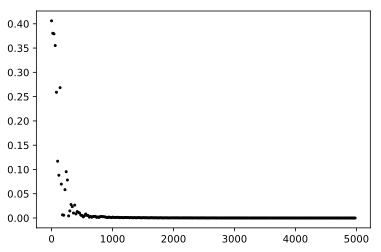
\includegraphics{output_0_11.pdf}
\end{center}

Widać wyraźnie, że sieć w tej konfiguracji nie jest w stanie zminimalizować błędu nawet po 500000 epok.

\subsubsection{Konfiguracja 4-3-3, 70000 epok}
\begin{center}
  \includegraphics{output_0_0.pdf}
\end{center}
\begin{center}
  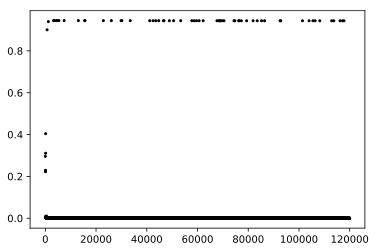
\includegraphics{output_0_1.pdf}
\end{center}

Zbiór walidacyjny: Maksymalny błąd: 0.994885, średni błąd: 0.070864.
Sieć poprawnie rozpoznała 33/38 kwiatów.

\subsubsection{Konfiguracja 4-7-3, 70000 epok}
\begin{center}
  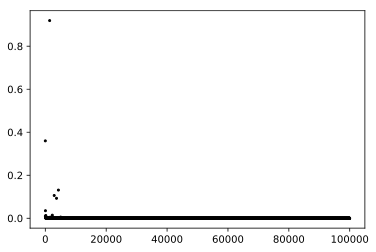
\includegraphics{output_0_3.pdf}
\end{center}
\begin{center}
  \includegraphics{output_0_4.pdf}
\end{center}

Zbiór walidacyjny: Maksymalny błąd: 0.016240, średni błąd: 0.000484.
Sieć poprawnie rozpoznała wszystkie kwiaty (34).

\subsubsection{Konfiguracja 4-5-4-3, 70000 epok}
\begin{center}
  \includegraphics{output_0_6.pdf}
\end{center}
\begin{center}
  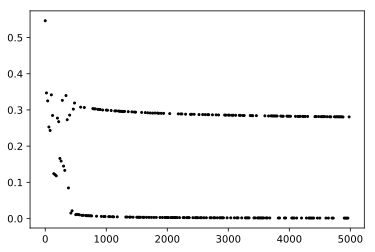
\includegraphics{output_0_7.pdf}
\end{center}

Zbiór walidacyjny: Maksymalny błąd: 0.984808, średni błąd: 0.038473.\newline
Sieć poprawnie rozpoznała 29/30 kwiatów.

\subsubsection{Konfiguracja 4-4-4-4-3, 70000 epok}
\begin{center}
  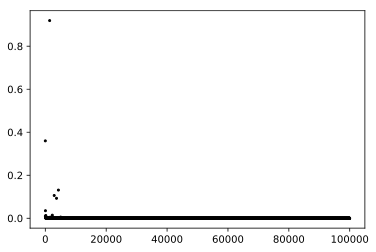
\includegraphics{output_0_3.pdf}
\end{center}
\begin{center}
  \includegraphics{output_0_4.pdf}
\end{center}


Zbiór walidacyjny: Maksymalny błąd: 0.997997, średni błąd: 0.064793.
Sieć poprawnie rozpoznała 32/34 kwiatów.

\newpage
\section{Wnioski}
Perceptron wielowarstwowy może z powodzeniem służyć jako klasyfikator irysów. Do realizacji tego zadania potrzeba skonfigurować sieć z przynajmniej jedną warstwą ukrytą - i ta ukryta warstwa w zupełności wystarcza.
\begin{thebibliography}{0}
  \bibitem{l2short}
    \textsl{http://archive.ics.uci.edu/ml/datasets/Iris}
\end{thebibliography}
\end{document}
